\documentclass[a4paper,12pt]{article}

%%% Работа с русским языком
\usepackage{cmap}					% поиск в PDF
\usepackage{mathtext} 				% русские буквы в фомулах
\usepackage[T2A]{fontenc}			% кодировка
\usepackage[utf8]{inputenc}			% кодировка исходного текста
\usepackage[english,russian]{babel}	% локализация и переносы

%%% Дополнительная работа с математикой
\usepackage{amsfonts,amssymb,amsthm,mathtools} % AMS
\usepackage{amsmath}
\usepackage{icomma} % "Умная" запятая: $0,2$ --- число, $0, 2$ --- перечисление

%% Номера формул
%\mathtoolsset{showonlyrefs=true} % Показывать номера только у тех формул, на которые есть \eqref{} в тексте.

\usepackage{hyperref}
\hypersetup{
    colorlinks=true,
    linkcolor=blue,
    filecolor=magenta,      
    urlcolor=cyan,
}

\usepackage{float}


%% Шрифты
\usepackage{euscript}	 % Шрифт Евклид
\usepackage{mathrsfs} % Красивый матшрифт

%%% Работа с картинками
\usepackage{graphicx}  % Для вставки рисунков
\graphicspath{{images/}{images2/}}  % папки с картинками
\setlength\fboxsep{3pt} % Отступ рамки \fbox{} от рисунка
\setlength\fboxrule{1pt} % Толщина линий рамки \fbox{}
\usepackage{wrapfig} % Обтекание рисунков и таблиц текстом
\usepackage{caption}
\usepackage{subcaption}
\captionsetup{labelsep=period} %. вместо : в рис

\title{Использование numba cuda jit}
\author{Москаленко Роман}
\date{}

\begin{document}

\maketitle

\section{Введение}
Игра Новака и Мэя в классическом виде, при синхронной игре и подсчёте очков агентов, позволяет проводить вычисления для агентов отдельно, независимо друг от друга. Значит моделирование игры можно проводить на GPU для большей эффективности. 

Были написаны две версии функции использующих numba.cuda.jit и соответственно работающих на GPU. Эти функции и будут разобраны ниже

\section{GPU и cuda}

Перед объяснением работы написанных функций, есть несколько основных понятий и принципов, на которых основывается cuda код.

\subsection{Блоки и потоки}

При каждом запуске cuda функции мы обозначаем количество блоков и потоков в блоках, на которых будут производиться вычисления.  Количество блоков и потоков может быть как числом, так и двумерным или трёхмерным массивом, соответственно массивы будут задавать форму сетки блоков и потоков. Каждый поток в блоке будет выполнят весь код написанный в функции, уникальность действий каждого потока достигается за счёт возможности получить номер потока (как внутри блока, так и во всей сетке). Аналогично в случае, когда количество потоков и блоков задаётся массивом, можно узнать координаты потока в заданной сетке. Количество потоков в одном блоке ограничено $\le 1024$

\subsection{Память}

У GPU есть несколько доступных видов памяти, однако нас интересуют глобальная память(global memory) и разделяемая память (shared memory).

Глобальная память позволяет нам хранить данные необходимые для вычислений на самом девайсе. Что значительно уменьшает время обращения к переменным, по сравнению с памятью хоста. Желательно перекинуть всё необходимое для вычислений в Глобальную память, это можно сделать вне cuda функции используя cuda.array.

Разделяемая память выделяется отдельно для каждого блока, все потоки в блоке имеют к ней доступ. Её очень мало (от 16 до 40 килобайт.). Время обращения к разделяемой памяти меньше чем к глобальной примерно в 100 раз. Поэтому если поток обращается к чему-то в глобальной памяти несколько раз, или если потоки в блоке обращаются к одним и тем же переменным в глобальной памяти, их стоит подгрузить в разделяемую память и дальше работать с ней.

\section{Функция для простой кубической решётки}

\subsection{Описание алгоритма}

Есть главная функция \verb|evolve3D_5|, из которой потом вызываются cuda функции. Тут же происходит выделение глобальной памяти

Две вспомогательные cuda функции нужны для избежания лишних действий с памятью хоста. Первая обнуляет переданный массив, вторая копирует элементы из первого массива во второй. эти функции используются на глобальных массивах. Без них пришлось бы использовать \verb|cuda_to_device| что сильно замедлит программу.

Основной код разбит на две функции \verb|culc_scores3D| и \verb|new_strategies3D|. Они написаны так, чтобы работать с трёхмерной сеткой блоков и потоков. Основная идея заключается в том, чтобы каждый блок подгружал, кубический кусочек поля в разделяемую память, затем мы работаем со всеми агентами, кроме крайних, так как для них в разделяемую память загружены все соседи. Блоки смещены так, чтобы соседние блоки пересекались по двум слоям агентов, в итоге крайние агенты каждого блока обрабатываются соседними блоками. Двумерная иллюстрация этого разбиения показана на рис. \ref{fig:blocks}

\begin{figure}[H]
	\centering
	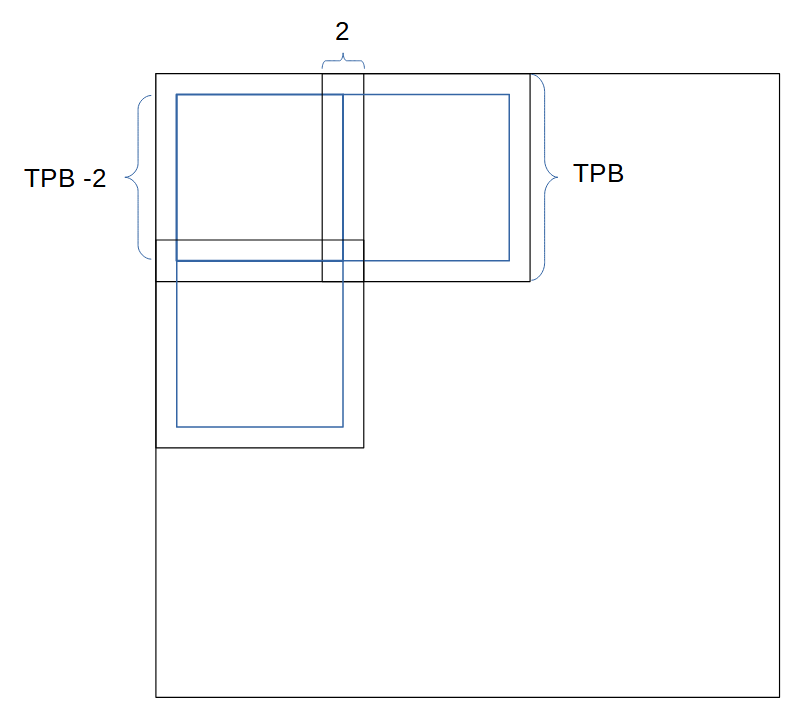
\includegraphics[width = 0.5\textwidth]{Images/Block visualisation.png}
	\caption{Пример расположения блоков на двумерном поле. TPB - threads per block количество потоков в блоке.}
	\label{fig:blocks}
\end{figure}

Подгрузка происходит в начале каждой функции (рис. \ref{fig:preloading}). Каждый поток загружает один, соответствующий элемент массива в shared memory. Затем следует команда cuda.sincthreads() которая означает, что потоки продолжат выполнение программы только, когда все потоки дойдут, до этой метки ( то есть когда все потоки подгрузят свой кусочек массива). Далее мы останавливаем все потоки, отвечающие за края блока. Остальной код аналогичен коду в функциях без использования cuda.

\begin{figure}[hbt]
	\centering
	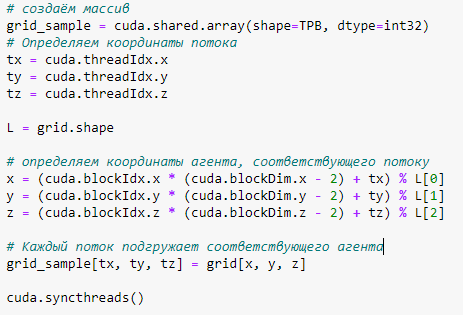
\includegraphics[scale=0.8]{Images/Подгрузка массива.png} 
	\caption{Часть кода в которой происходит загрузка данных в разделяемую память}
	\label{fig:preloading}
\end{figure}

В \verb|culc_scores3D| мы подгружаем часть массива grid, а в \verb|new_stratagies3D| часть массива scores. Так как для обработки одного агента, каждому потоку в функциях нужно обратиться к соответствующим массивам 27 раз. Остальные массивы подгружать не имеет смысла, так к ним потоки обращаются 1 раз.



\subsection{Время работы}

Данная функция показала наилучшее время. Она превосходит Cython и Numba. 

% Графики
\begin{figure}[H]
	\centering
	\begin{subfigure}[b]{0.45\textwidth}
		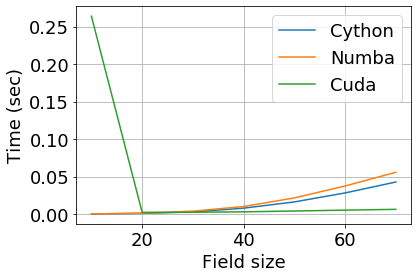
\includegraphics[width = \textwidth]{Images/1_step_time_with_cuda.png}
		\caption{Врема расчёта одного шага эволюции} 
	\end{subfigure}
	\hfill
	\begin{subfigure}[b]{0.45\textwidth}
		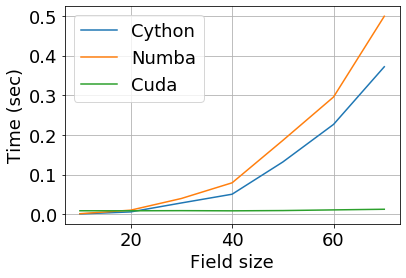
\includegraphics[width = \textwidth]{Images/10_step_time_with_cuda.png} 
		\caption{Врема расчёта десяти шагов эволюции} 
	\end{subfigure}
	\caption{Графики времени работы различных реализаций функции}
\end{figure}

При увеличении количества шагов эволюции время работы меняется незначительно и не линейно. Это связанно с тем, при каждом вызове функции массив с полем переносится на девайс и обратно, и это занимает большое количество времени. Для частых замеров можно переписать функцию так, чтобы перенос массива происходил вне функции, что позволит загрузить поле на девайс один раз, и затем загружать его с девайса на хост, чтобы получить результаты. Это должно сократить время работы на маленьком количестве шагов примерно в 2 раза.




\section{Функция с таблицей соседей}

Без использования GPU наилучшие время работы достигалось функциями, использующими заранее подготовленные таблицы соседей: массивы в которых для каждого агента записаны номера всех его соседей. Эти таблицы позволяли избежать лишних арифметических операций и заменить их одним обращением к памяти. Так же использование таблиц делало функцию универсальной, позволяя использовать её на полях любой формы.

Вторая вариация функции evolve3D\_ 4 с numba.cuda так же основывалась на таблицах соседей. Функция должна была быть универсальной и работать с полями другой формы или с другим расположением соседей. По структуре она идентична evolve3D\_ 5 с одной главной функцией и четырьмя cuda функциями. Но в данном случае использование таблицы соседей не даёт выигрыша в скорости.

\begin{figure}[H]
	\centering
	\begin{subfigure}[b]{0.45\textwidth}
		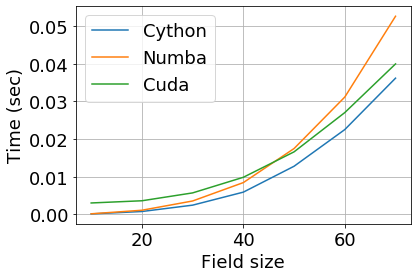
\includegraphics[width = \textwidth]{Images/1_step_universal_cuda.png} 
		\caption{Врема расчёта одного шага эволюции} 
	\end{subfigure}
	\hfill
	\begin{subfigure}[b]{0.45\textwidth}
		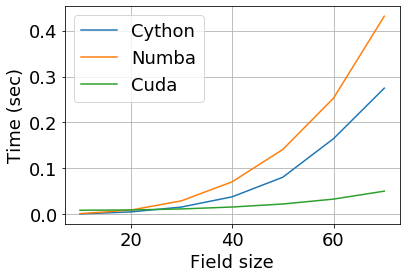
\includegraphics[width = \textwidth]{Images/10_step_universal_cuda.png} 
		\caption{Врема расчёта десяти шагов эволюции} 
	\end{subfigure}
	\caption{Графики времени работы различных реализаций функции}
\end{figure}

Замедление функции связано с тем, что теперь помимо массива агентов, на девайс нужно загрузить таблицу соседей. Это занимает более 90\% времени работы (рис. \ref{fig:0_steps}). Для конкретных замеров на малых временах это можно так же как и в предыдущем случае, производя загрузку вне функции.

\begin{figure}
	\centering
	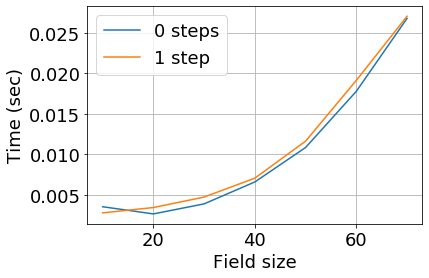
\includegraphics[width = 0.5\textwidth]{Images/0_and_1_step_time.png} 
	\caption{Время работы \texttt{evolve3D\_4} на одном шаге и 0 шагах эволюции. Во втором случае получается время загрузки массивов на девайс}
	\label{fig:0_steps}
\end{figure}

Так же если рассмотреть время работы функции на большом количестве шагов эволюции (рис. \ref{fig:1000_step_ratio}), где загрузка массивов уже не составляет большую часть времени работы, видно что \verb|evolve3D_4| Всё ещё медленнее чем \verb|evolve3D_5|.

\begin{figure}[hbt]
	\centering
	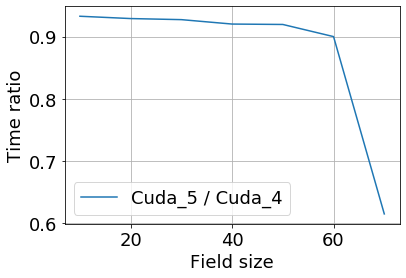
\includegraphics[width = 0.5\textwidth]{Images/Cuda_5_to_Cud_4_on_1000_step.png} 
	\caption{Отношение времени работы функции для кубической решётки к времени работы функции с таблицей соседей на 1000 шагов}
	\label{fig:1000_step_ratio}
\end{figure}

Это происходит из-за более частых обращений к глобальной памяти девайса. Помимо того, что в данном решении, чтобы узнать стратегию или счёт соседа нам необходимо 2 обращения, но и из-за того, что функция должна быть универсальной, нет простого способа использовать разделяемую память.

В \verb|evolve3D_5| благодаря известной форме поля и расположению соседей мы можем использовать информацию, подгруженную потоками из одного блока. Однако для поля общего вида с таблицей соседей очень сложно разбить агентов на блоки так, чтоб соседи находились в одном блоке, и  разделить подгрузку информации об агентах между потоками внутри блока. В итоге в то время как в функциях исполняемых на CPU, используя таблицу соседей, мы заменяли 6 арифметических операций одним обращением к памяти, на GPU мы ,избавляясь от тех же 6 операций, получаем 26 обращений к памяти.



\section{Заключение}
В готовом виде простая замена функции с cython на любую из разобранных функций, на большом количестве шагов уменьшит время работы примерно в 50 раз (рис. \ref{fig:cython_ratio}). Для замеров на малых временах необходима небольшая доработка кода вне функции, для предварительной загрузки информации о поле на девайс.

\begin{figure}[htb]
	\centering
	\begin{subfigure}[b]{0.45\textwidth}
		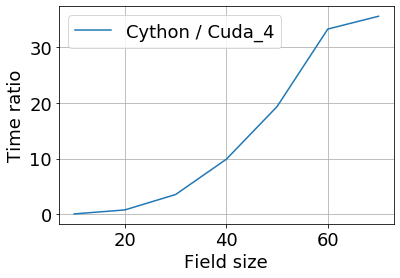
\includegraphics[width = \textwidth]{Images/Cython_to_cuda4_on_1000_step.png} 
		\caption{\texttt{evolve3D\_4}}
	\end{subfigure}
	\hfill
	\begin{subfigure}[b]{0.45\textwidth}
		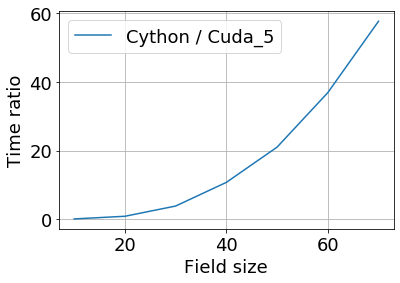
\includegraphics[width = \textwidth]{Images/Cython_to_Cuda5_on_1000_step.png}
		\caption{\texttt{evolve3D\_5}} 
	\end{subfigure}
	\caption{Отношение времени работы cuda функций к времени работы cython функции на 1000 шфгов эволюции}
	\label{fig:cython_ratio}
\end{figure}

\end{document}
